
This chapter presents the optimization development. Topics such as algorithm configuration, choice of design variables and definition of constraints and objective function will be addressed.

\section{Problem Definition}

The problem definition is to find a controller design that provides increased actuation system dynamic stiffness when compared to an initial provided controller while respecting the performance requirements of the system. In this work, four classical controllers were considered, hence, the optimization was performed for each of them.

As explained in Section \ref{2-4-3-SelectedAlgorithm} this optimization is constrained, nonlinear, continuous, deterministic and single objective. Despite the small number of design variables, this is a complex problem because of its high computational cost which will be discussed in the following sections.

The problem is described by Equations \ref{eq:2_2_OptimizationFormulation} to \ref{eq:2_2_BoundsOptimizationFormulation}. The objective function $f(x)$ is described in section \ref{4-4-ObjectiveFunction}, the constraitn function $g(x)$ is presented in Section \ref{4-3-ConstraintFunction} and the design variables $x$, it boundaries and other optimization parameters are presented in Section \ref{4-2-OptimizationParameters}. The equality constraint function $h(x)$ does not apply to this problem, hence it will not be considered. 

An algorithmic program was developed to structure the optimization problem solution in an organized and user friendly manner. A high level flowchart of the program is presented in Figure \ref{fig:4_1_MainFlowchart}.

\begin{figure}[H]
	\centering
	\centerline{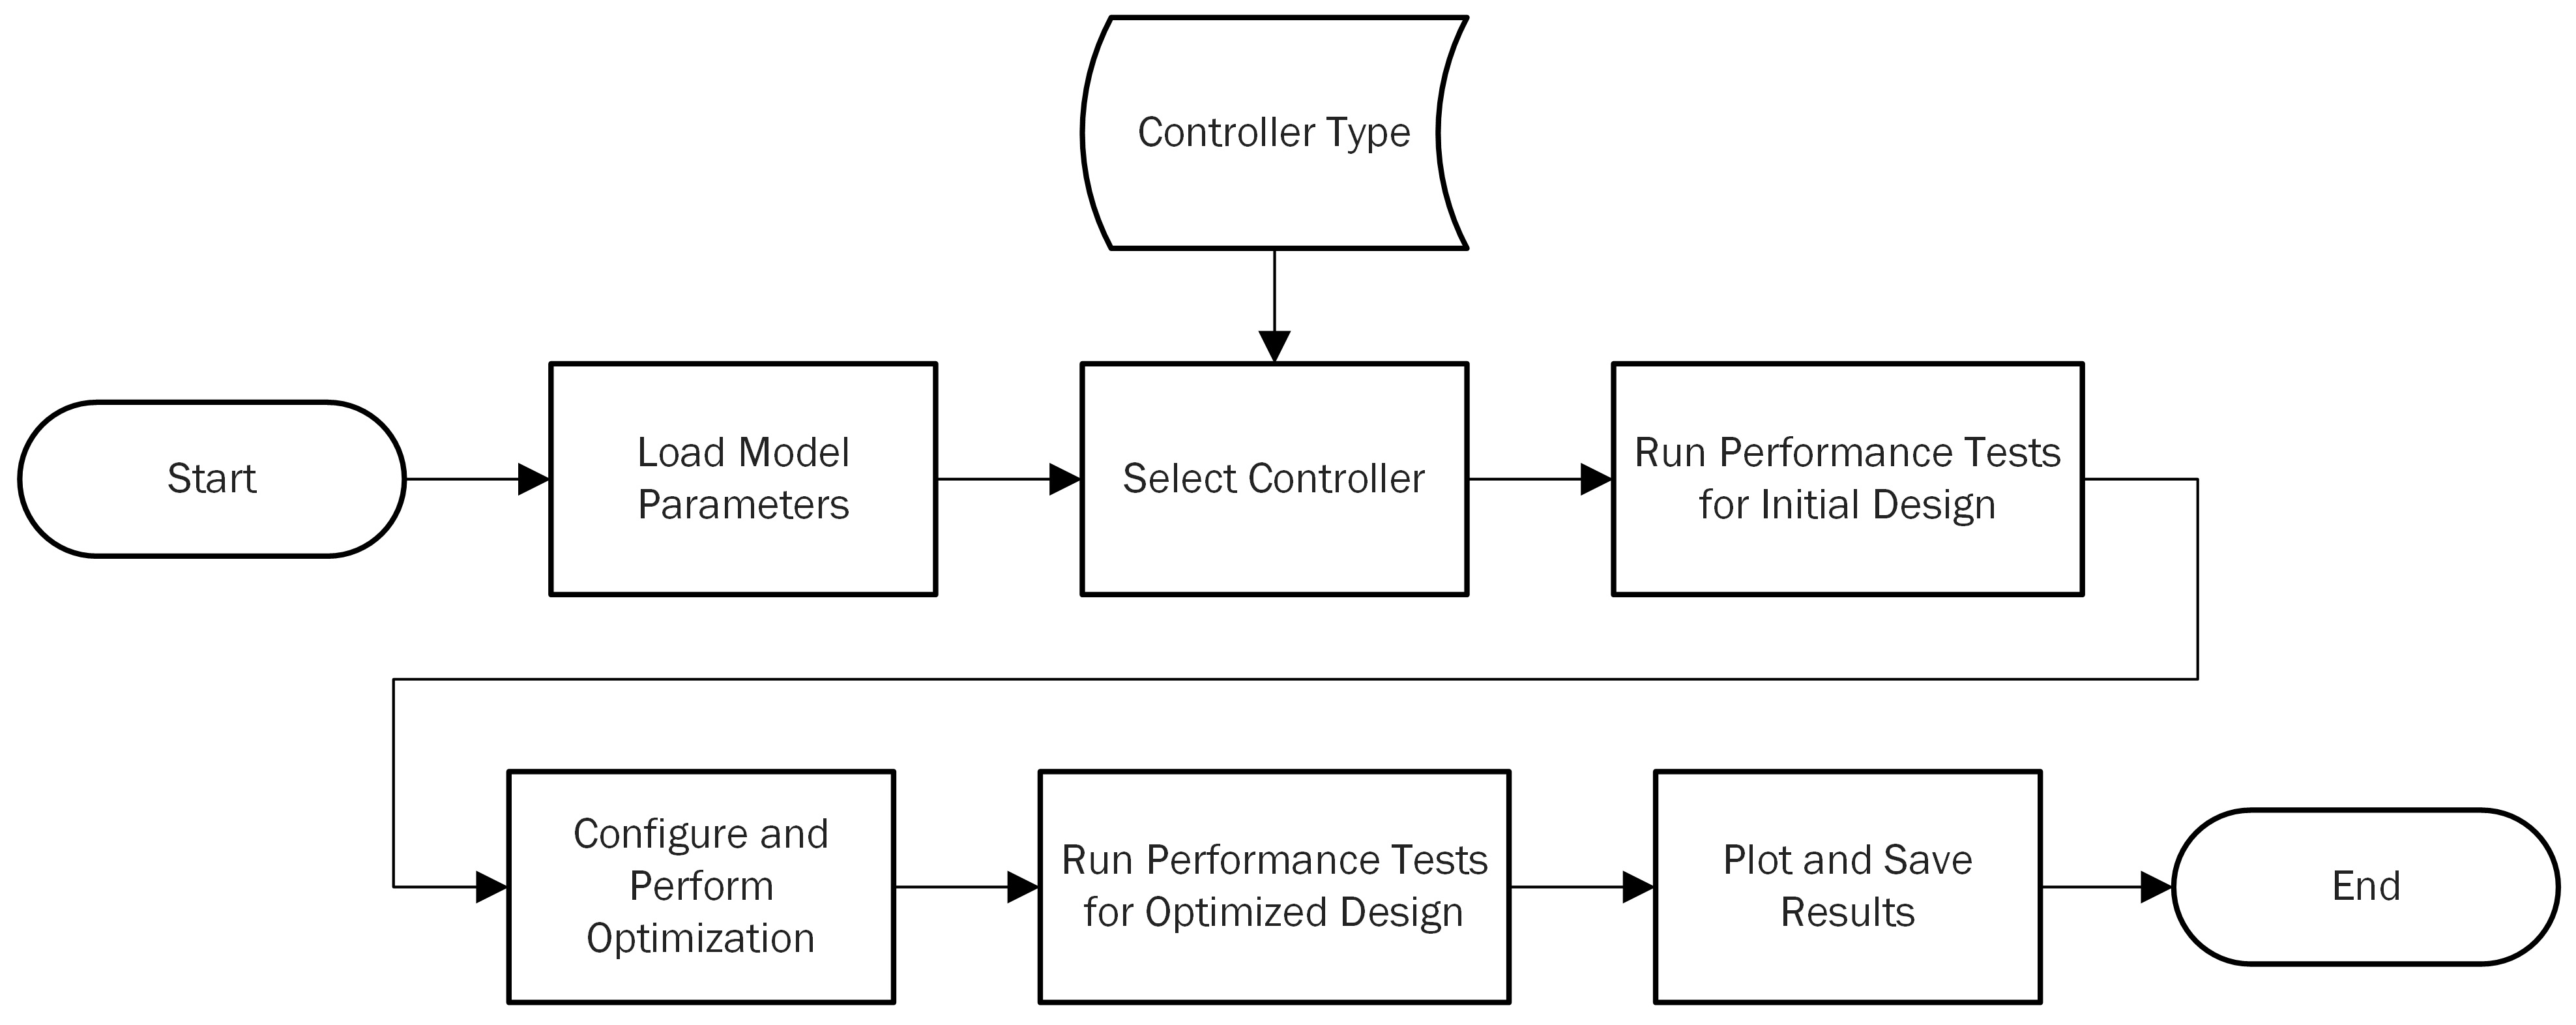
\includegraphics[width=0.9\textwidth]{Figuras/4.DynamicStifinessOptimizationAlgorithm/4-1-MainFlowchart.jpg}}
	\caption{Program Flowchart}
	\label{fig:4_1_MainFlowchart}
\end{figure}

The program starts by clearing the workspace and initializing parameters of the model presented in Chapter \ref{Actuation System Model}. These include the physical dimensions valves, cylinder and rod as well as hydraulic fluid characteristics and simulation parameters.

After that, the user selects the controller type to be evaluated using a dialog box. Next, the initial solution performance is evaluated with dynamic stiffness, step response and frequency response tests and the results saved for future comparison with optimized design.

The next step is configuring and performing the optimization itself, where the chosen solver, \textit{fmincon}, iteratively updates controller gains while evaluating objective and constraint functions. After optimization, dynamic stiffness, step response and frequency response tests are performed with the optimized controller and finally the results are plotted into graphs and saved in the hard drive.

The following sections will present in detail the optimization configuration, the constraints and the objective function.

\section{Optimization Settings} \label{4-2-OptimizationParameters}

This section will present the settings used to solve the optimization problem. 

One of them is the optimization method employed. In this case, as discussed in Section \ref{2-4-3-SelectedAlgorithm}, the Interior Point algorithm was selected. This method needs few function evaluations to converge and is therefore suitable for problems with long execution time.

The design variables $x$ defined for this problem are the gains of the control architecture being evaluated. This is a natural definition that comes from the parametric study performed by \citeonline{Ballesteros} which observed the influence of such gains in the actuation system dynamic stiffness response. 

The range of these design variables that will be considered as possible solutions to the problem can be bounded as per Equation \ref{eq:2_2_BoundsOptimizationFormulation}. Through the correct definition of these boundaries it is possible to improve algorithm convergence and also to reduce execution time since the space of possible solutions will be smaller.

These boundaries have been defined considering the mentioned study performed by \citeonline{Ballesteros}. It evaluated the performance of the actuation system for a broad range of proportional, integral and derivative gain values. The gain values that yielded unstable actuation systems or ones that did not comply with performance requirements were discarded. The lower and upper boundaries selected are shown in Table \ref{table:4_2_ControllerGainBoundaries}.

\begin{table}[H]
	\captionof{table}{Classic Controller Gain Boundaries}
	\label{table:4_2_ControllerGainBoundaries}
	\centering
	\resizebox{8cm}{!} {
		\begin{tabular}{|l|c|c|}
			\hline
			Parameter & Lower Boundary ($x_l$)  & Upper Boundary ($x_u$)\\ \hline
			$K_p$ 	  & $10$  		   			& $100$ 				\\ \hline
			$K_i$ 	  & $0$  		   			& $5$ 					\\ \hline
			$K_d$ 	  & $0$  		   			& $5$	 				\\ \hline
	\end{tabular}}
\end{table}

Also, stopping criteria tolerances were defined for the design variables, constraints and objective function. Based on these definitions, the optimization program stops when the changes in these parameters are smaller than the tolerance values.  These values were defined empirically during development because they depend on the magnitude of these parameters. Table \ref{table:4_2_StoppingCriteriaParam} shows their final values.

\begin{table}[H]
	\captionof{table}{Stopping Criteria Parameters}
	\label{table:4_2_StoppingCriteriaParam}
	\centering
	\resizebox{6cm}{!} {
		\begin{tabular}{|l|c|c|}
			\hline
			Parameter 			  & Tolerance Value \\ \hline
			Objective Function 	  & $1e-6$	  \\ \hline
			Design Variable 	  & $1e-4$	  \\ \hline
			Constraint		  	  & $1e-4$	  \\ \hline
	\end{tabular}}
\end{table}

\section{Optimization Constraints} \label{4-3-ConstraintFunction}

The constraint function $g(x)$ is designed to incorporate the time and frequency domain performance requirements that are usually applied to rudder surface actuation systems. Table \ref{table:4_3_ConstParam} shows the considered performance parameter as well as their respective requirements.

\begin{table}[H]
	\captionof{table}{Constraints Parameters}
	\label{table:4_3_ConstParam}
	\centering
	\resizebox{9cm}{!}{
		\begin{tabular}{|l|c|}
			\hline
			Performance Parameter						& Requirement 	\\ \hline
			Settling Time (ms) 			 				& $< 1100$  	\\ \hline
			Steady State Error (\%) 	 				& $< 1$ 		\\ \hline
			Overshoot (\%) 				 				& $< 10$ 		\\ \hline
			Minimum Average Rate ($°$/s) 				& $> 32$ 		\\ \hline
			Maximum Average Rate ($°$/s) 				& $< 36$ 		\\ \hline
			Closed-Loop Gain Allowance (dB) 			& $> 10$	 	\\ \hline
			Closed-Loop Phase Allowance ($°$)			& $> 45$ 		\\ \hline
			Closed-Loop Maximum Peak (dB) 				& $< 0.5$ 		\\ \hline
	\end{tabular}}
\end{table}

The requirements used in this work are similar to those proposed by Ballesteros (2015). However, there are two differences: the maximum magnitude requirement was introduced and in this work, the settling time requirement is 1100 ms, instead of 850 ms.

The maximum magnitude requirement was introduced to limit eventual peaks in the magnitude frequency response. High peaks are not desired because they are related to poor dynamic stiffness at the frequency of the peak \cite{Ballesteros}.

To obtain the settling time, the step time instant is subtracted from the instant when model response reaches and remains within $\pm2\%$ of its steady-state value. The settling times presented in the results of \citeonline{Ballesteros} subtracted twice the step time instant instead of one. This reduced all settling times by 250ms what made the 850ms requirement of that work feasible. 

To enable a fair comparison with previous results, the settling time requirement considered in this development is 1100 ms, which is the previous requirement plus 250ms of the step time instant.

The step response is obtained for a maximum deflection scenario, in which the actuator initial position is neutral and the final position is the nominal mechanical stop of the piston. This condition is more conservative because the actuator load is always against the movement and thus requiring more effort from the actuation system. The numerical definition of the step will be presented in the following sections.

The frequency domain performance parameters are all obtained from the closed-loop frequency response which is the response of the complementary sensitivity function (Equation \ref{eq:2_2_2_CompSensitivityTF}). As explained in Section \ref{2-4-3-SelectedAlgorithm}, it is not practical to specify the loop transfer function parameters and therefore the industry approach will be followed in this development.

The frequency response is obtained through model simulations with a sinusoidal input. The response in obtained from the surface command in degrees to the actuator piston position converted from millimeters to degrees. Also, the surface degrees command amplitude must be one that does not lead to a saturation of the servo valve current command.

The constraint parameters are obtained by simulating step and frequency response tests in the actuation system Simulink model. These tests are described in the following sections.

\subsection{Step Response Test} \label{4-3-1-StepRespTest}

The step response test is simple and its execution sequence is described in Figure \ref{fig:4_3_1_TimeResponseFlowchart}.  

\begin{figure}[H]
	\centering
	\centerline{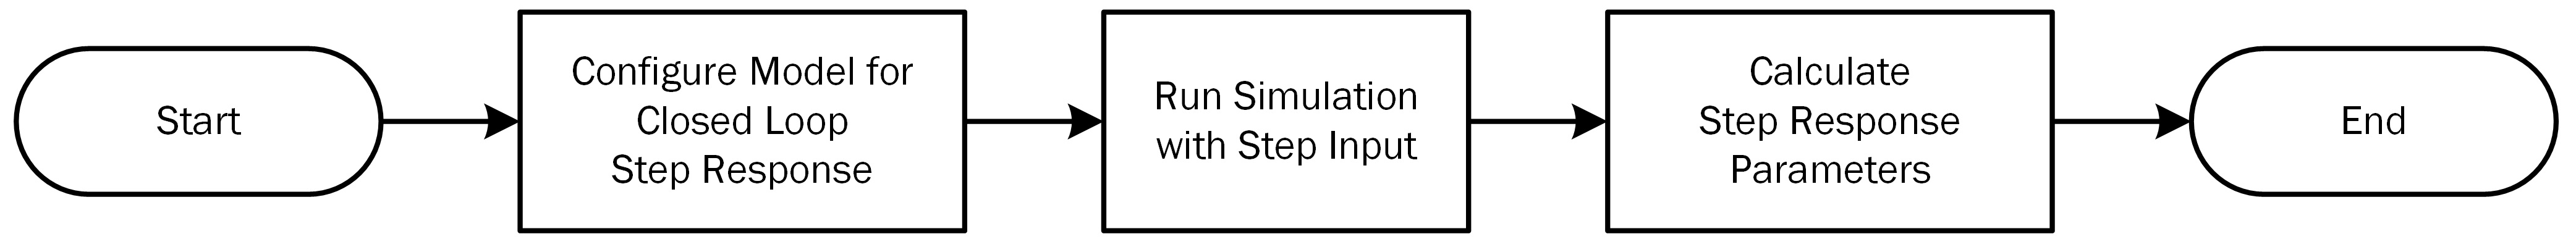
\includegraphics[width=0.9\textwidth]{Figuras/4.DynamicStifinessOptimizationAlgorithm/4-3-1-TimeResponse.jpg}}
	\caption{Step Response Test Flowchart}
	\label{fig:4_3_1_TimeResponseFlowchart}
\end{figure}

Initially, the model is configured to match the following test conditions:

\begin{enumerate}[a)]
	\item Single actuator connected to rudder surface;	
	\item Initial position = 0$°$;
	\item Step amplitude = 30$°$;	
	\item Opposing hinge moment load varying linearly from 0 N.m to 3050 N.m;	
	\item Maximum hydraulic supply pressure of 3000 psi;
	\item Maximum hydraulic return pressure of 150 psi;	
	\item At -15$°C$ (5$°F$) fluid temperature.
\end{enumerate}

The test is performed with one actuator because the surface is required to maintain performance even with the other actuators failed. Also, the opposing hinge moment load profile refers to equivalent aerodynamic forces in rudder surfaces for the actuator sizing of this study. 

Additionally, the step amplitude is 30$°$ because that is the common deflection range of a rudder surface. It is important to evaluate time domain performance in a maximum deflection scenario due to critical events that may occur that require prompt surface response such as the loss of one engine or other thrust asymmetry scenario.

Typical fluid temperature operational envelope of the actuation system is between -15$°C$ and 100$°C$. Despite this, the step response is evaluated only at -15$°C$ because the actuation rate decreases when temperature falls what makes this condition the most conservative to evaluate settling time, steady state error and the actuation average rate.

At higher temperatures, fluid density and bulk modulus decrease and each one has a different effect in actuation rate. Lower fluid density leads to higher flow and as a consequence higher pressure at cylinder chambers, what increases actuation rate. On the other hand, lower bulk modulus increases fluid compressibility, leading to less pressure for the same volume and flow, what decreases actuation rate. 

However, the effect of decreasing fluid density is greater than the effect of a lower bulk modulus and, therefore, actuation rate will increase with fluid temperature. Figure \ref{fig:4_3_1_FluidTemperature} illustrates this behavior.

\begin{figure}[H]
	\centering
	\centerline{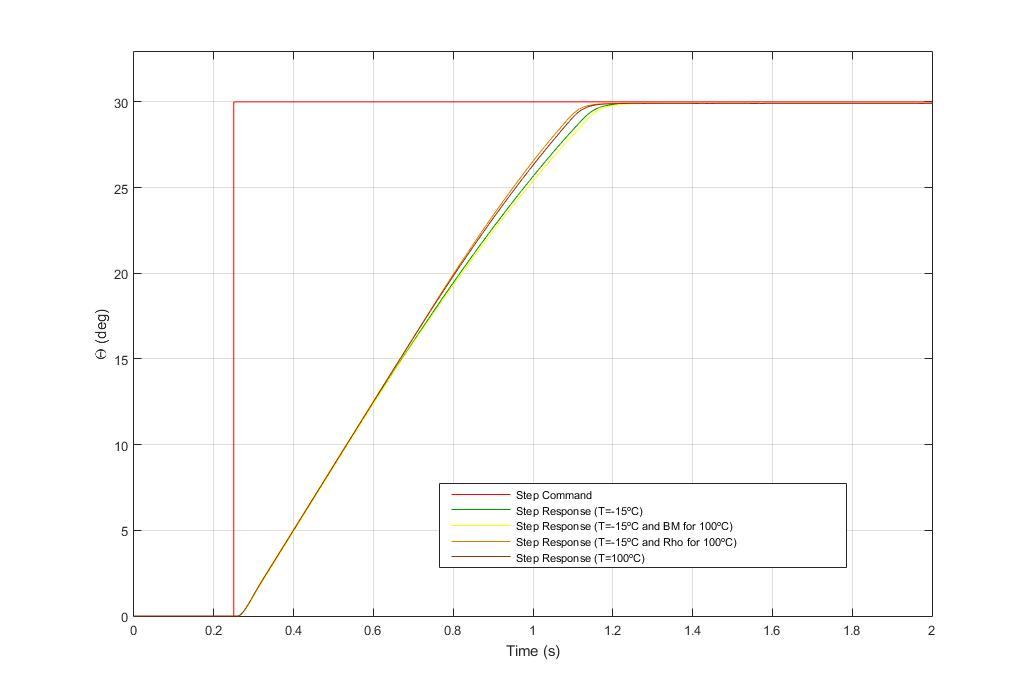
\includegraphics[width=0.9\textwidth]{Figuras/4.DynamicStifinessOptimizationAlgorithm/4-3-1-FluidTemperature.jpg}}
	\caption{Fluid Density and Bulk Modulus Contribution to Step Response Actuation Rate}
	\label{fig:4_3_1_FluidTemperature}
\end{figure}

Because higher actuation rates lead to overshoot, it is more conservative to evaluate this parameter at higher fluid temperatures. However, overshoot is associated with dynamic stiffness reduction \cite{Ballesteros} and, since the optimization will focus in increasing dynamic stiffness, it is expected that solutions that increase overshoot are avoided by the optimization algorithm. Also, since the actuation system model does not consider the control surface inertia only small overshoots are expected.

Therefore, evaluation at 100$°C$ is not performed to save execution time. Nevertheless, the final design step response will be obtained for both envelope corner temperatures, assuring average actuation rate and overshoot requirement compliance.

Additionally, it is advised to evaluate these constraints at 100$°C$ in a future work if the control surface dynamics is considered. In this case, the fluid temperature and the inertia will lead to an overshoot increase that will need to be avoided during optimization.

After parameter configuration, the test is performed and the following performance parameters are calculated:

\begin{enumerate}
	\item Settling time $t_{ss} < 1100 $ms;
	\item Steady state error $< 1\%$ of actuator full stroke;
	\item Overshoot $< 10\%$ of actuator full stroke;
	\item Average rate $> 32^{\circ}/s$;
	\item Maximum rate $< 36^{\circ}/s$.
\end{enumerate}

\subsection{Frequency Response Test} \label{4-3-2-FreqRespTest}

The frequency response is obtained through a series of model simulations, one for each evaluated frequency, and further processing of the data generated by these simulations. Figure \ref{fig:4_3_2_FrequencyResponseFlowchart} shows the flowchart of this test.

First, the model is configured to obtain a closed-loop frequency response in the following conditions:

\begin{enumerate}[a)]
	\item Closed-loop control configuration;
	\item Measured from the surface angular position command in degrees provided at the actuator controller digital input to the Actuator Ram Position Feedback converted to
	surface angular position in degrees;
	\item Single actuator connected to rudder surface;	
	\item Sinusoidal commands of 0.5{$°$} amplitude;	
	\item Without the presence of aerodynamic load and backlash;	
	\item For an actuator within nominal tolerances;
	\item At 100$°C$ (212$°F$) fluid temperature.	
\end{enumerate}

The fluid temperature is set to 100$°$C, which is the highest envelope temperature. Simulations performed during this development show that at this temperature the gain and phase allowances are smaller than these allowances at -15$°$C, thus evaluating this condition is a conservative approach for actuator design.

Next, the sine input frequency to be evaluated is selected and the simulation duration period is calculated. For frequencies up to 1 Hz, the duration spans for 3 complete input cycles and, for frequencies between 1 Hz and 35 Hz, the number of cycles covered by the simulation is 3 times the evaluated frequency. For instance, when evaluating the actuation system at 20 Hz, the simulation spans for 60 complete cycles.

\begin{figure}[H]
	\centering
	\centerline{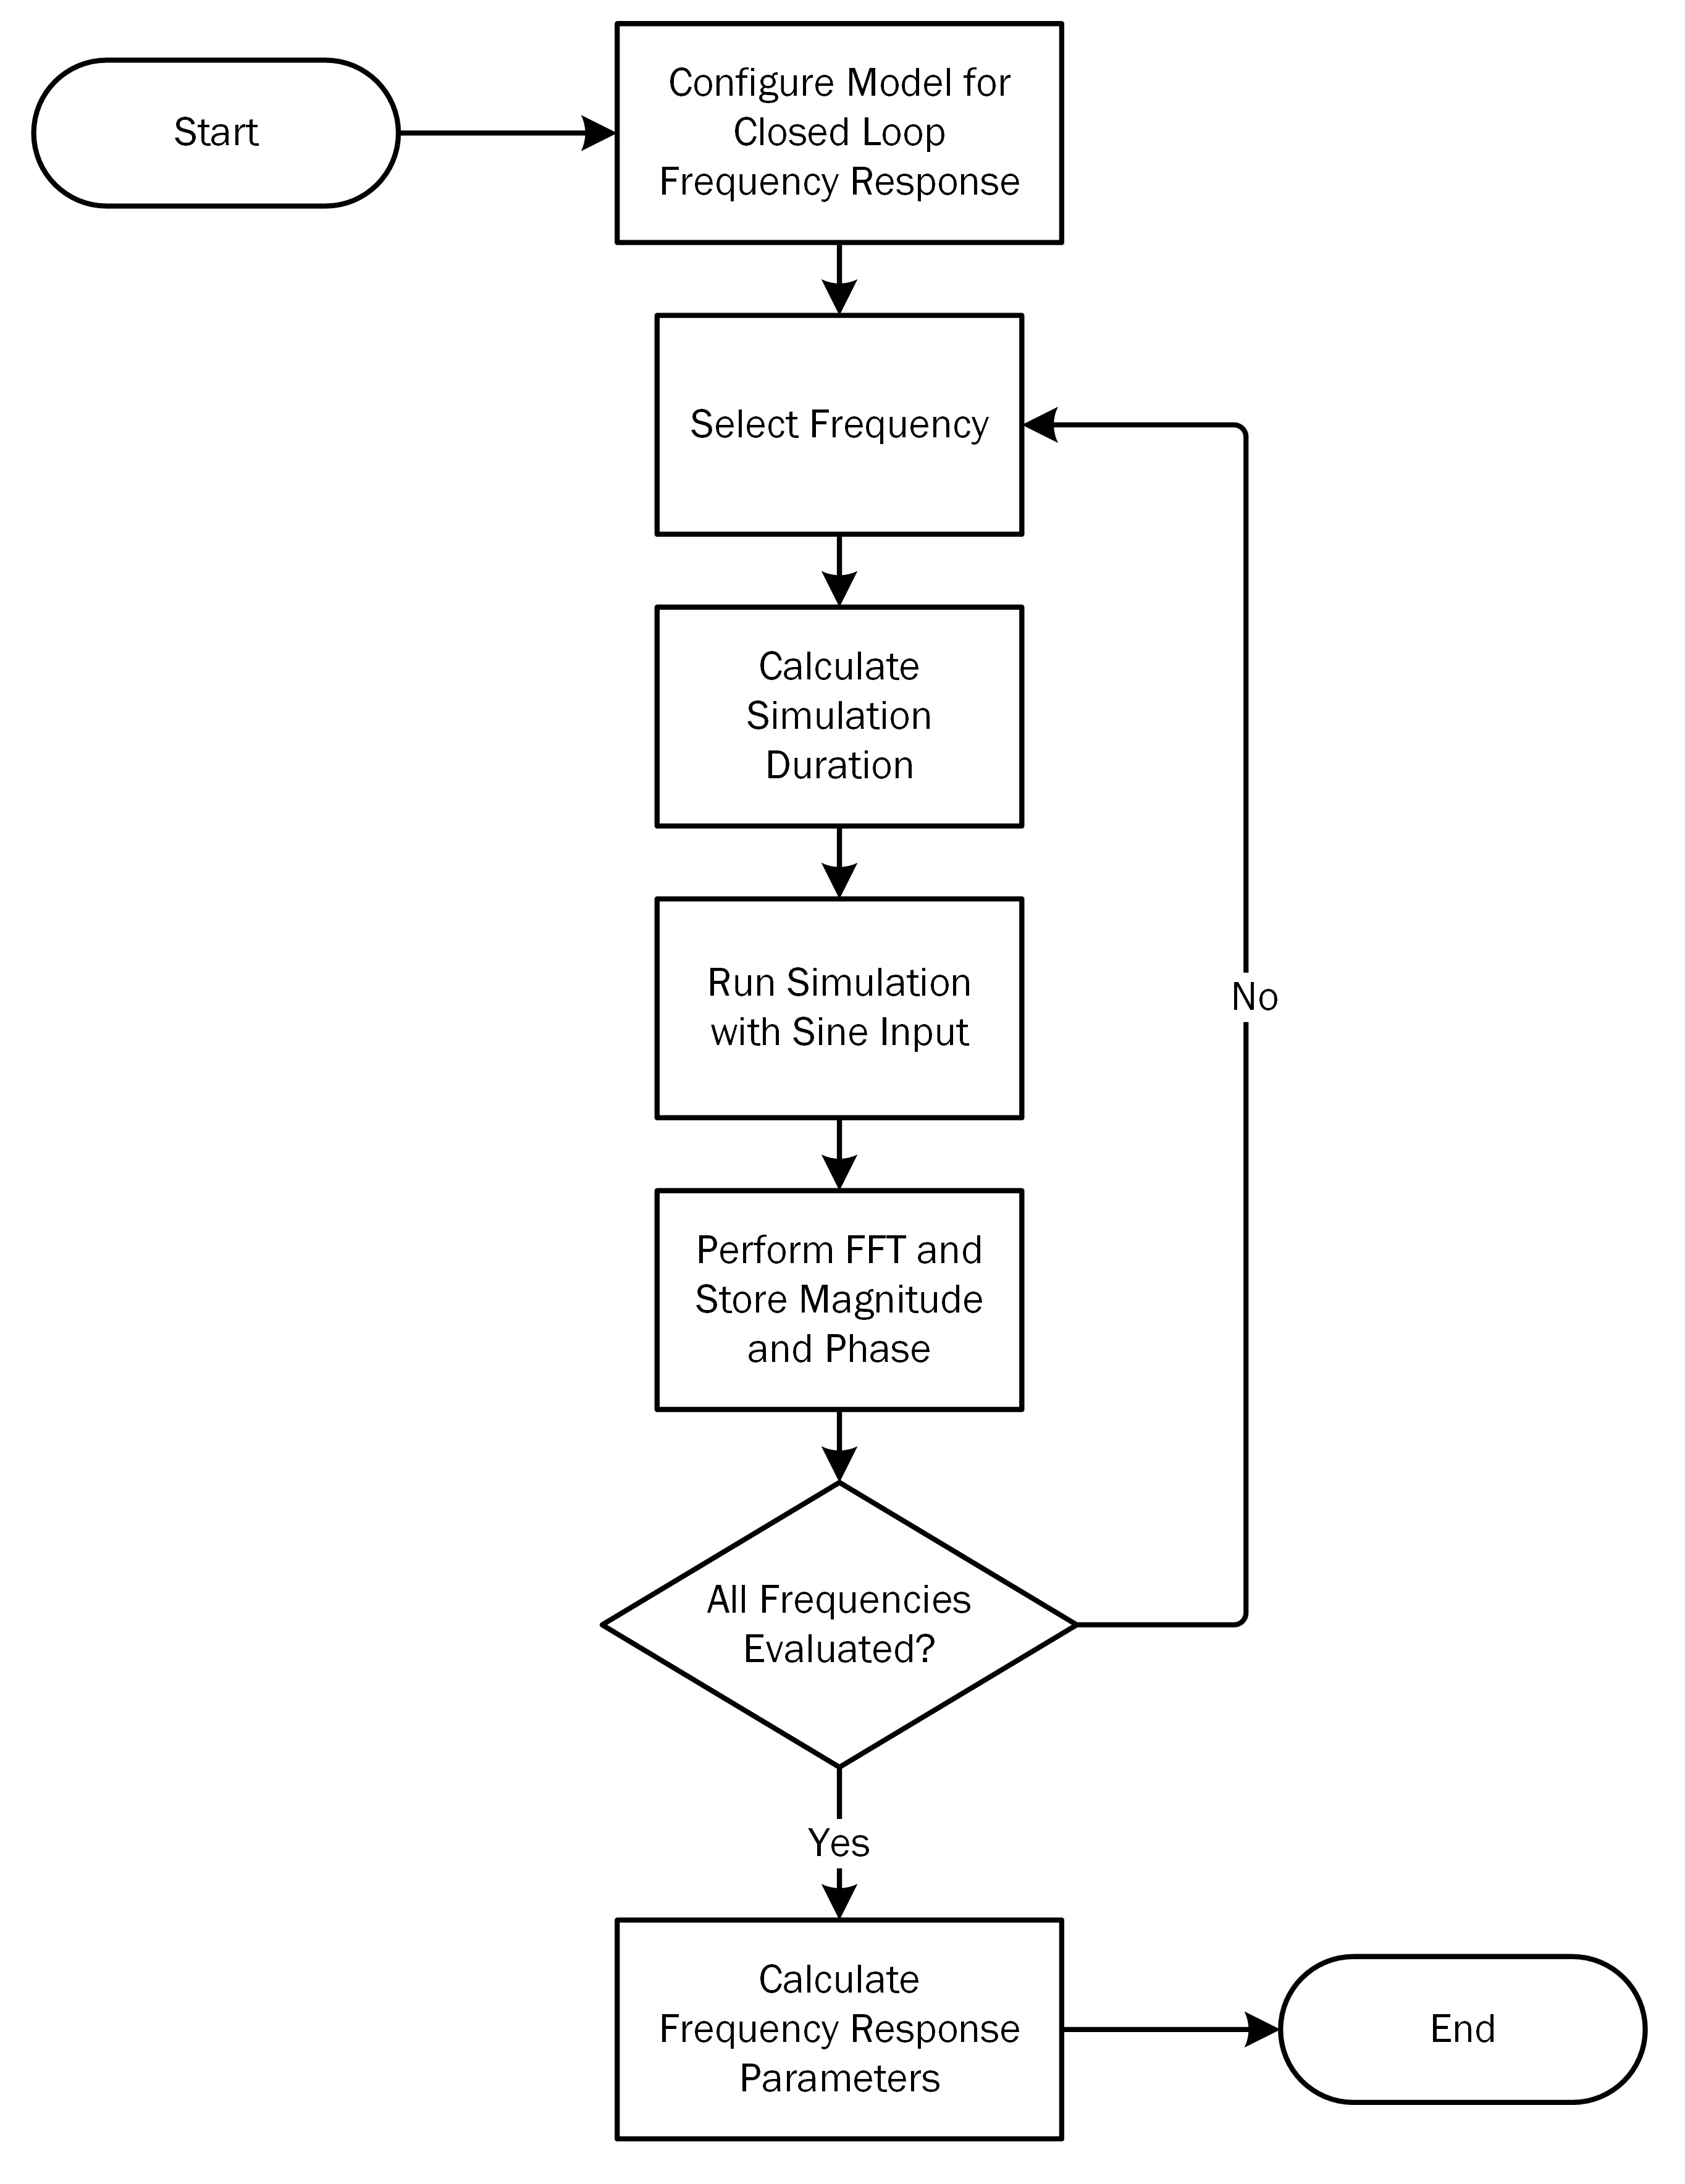
\includegraphics[width=0.6\textwidth]{Figuras/4.DynamicStifinessOptimizationAlgorithm/4-3-2-BaselineFrequencyResponse.jpg}}
	\caption{Flowchart of Baseline Frequency Response Test}
	\label{fig:4_3_2_FrequencyResponseFlowchart}
\end{figure}

After that, the simulation is performed and the sine input and surface position values are stored. This information is processed in the next step, when a Fast Fourier Transform (FFT) is performed for both simulation input and output considering all simulation time. The transformed vectors are manipulated and at this stage the magnitude and phase at the excitation frequency are stored. The last steps are repeated for all frequencies of interest until the magnitude and phase responses are complete. Finally, the performance parameters are obtained from these responses through Equations \ref{eq:2_2_2_MaxTSko}, \ref{eq:2_2_3_CLGainMargin} and \ref{eq:2_2_3_CLPhaseMargin}.

The execution time of this test is approximately 12 minutes but it depends on many factors such as the computer configuration, applications in execution and the model itself. During this development, when the frequency response constraints were implemented, it was noticed that this computational cost would lead to days of optimization execution what would eventually reduce the advantages of performing the optimization. 

Execution time is critical in optimization algorithms because of their iterative nature. The frequency response test describe above, referred later on as \textit{baseline}, is executed several times in a single run of the optimization program and its execution time can represent more than two hours altogether. If global optimization techniques are used, the frequency response algorithm can represent days of execution time.

To minimize this computational cost, other methods for obtaining the frequency response were studied as presented in Appendix A. The investigation on alternative methods resulted in a modification of the \textit{baseline} frequency response test that is presented below.

\subsubsection{Modified Frequency Response Test}

Since the execution time of the baseline test is mostly the time to execute all simulations, their duration was revisited. Instead of calculating simulation's length only from input signal cycles, a non variable time parameter was introduced with the aim to capture model dynamics settling time. The duration of each simulation was calculated with Equation \ref{eq:4_3_2_3_SimulationDuration}.

\begin{equation}
\label{eq:4_3_2_3_SimulationDuration}
T\textsubscript{sim} = T\textsubscript{dyn} + K\textsubscript{int} \times T_p
\end{equation}

$T\textsubscript{sim}$ is the simulation duration for each frequency whereas $T\textsubscript{dyn}$ is the model dynamics settling time. This constant parameter was obtained empirically from measuring the amplitude of actuator surface position in simulations with sine input for several frequencies which yielded a 0.5 seconds dynamics settling time. 

Parameter $K\textsubscript{int}$ is the number of integration cycles for the respective frequency and $T_p$ is the frequency's period. $K\textsubscript{int}$ was selected to minimize simulation time but in a way that did not jeopardize the frequency response. Frequencies 0.1, 0.5 and 1 Hz were integrated for only one cycle while three cycles were considered for 2 and 3 Hz and nine cycles for frequencies from 4 to 35 Hz. 

Figure \ref{fig:4_3_2_1_20HzTimeResponse} shows an example of the actuation system response for a 20 Hz sine input in which the orange curve shows approximately how the output amplitude behaves. It can be observed that dynamics of the model in the beginning of the simulation disappear after approximately 0.2 seconds, when the actuator response reaches a steady value. Even though the dynamics settling time is less than 0.2 seconds, a generous margin was allowed and a settling time of 0.5 seconds was considered.

\begin{figure}[H]
	\centering
	\centerline{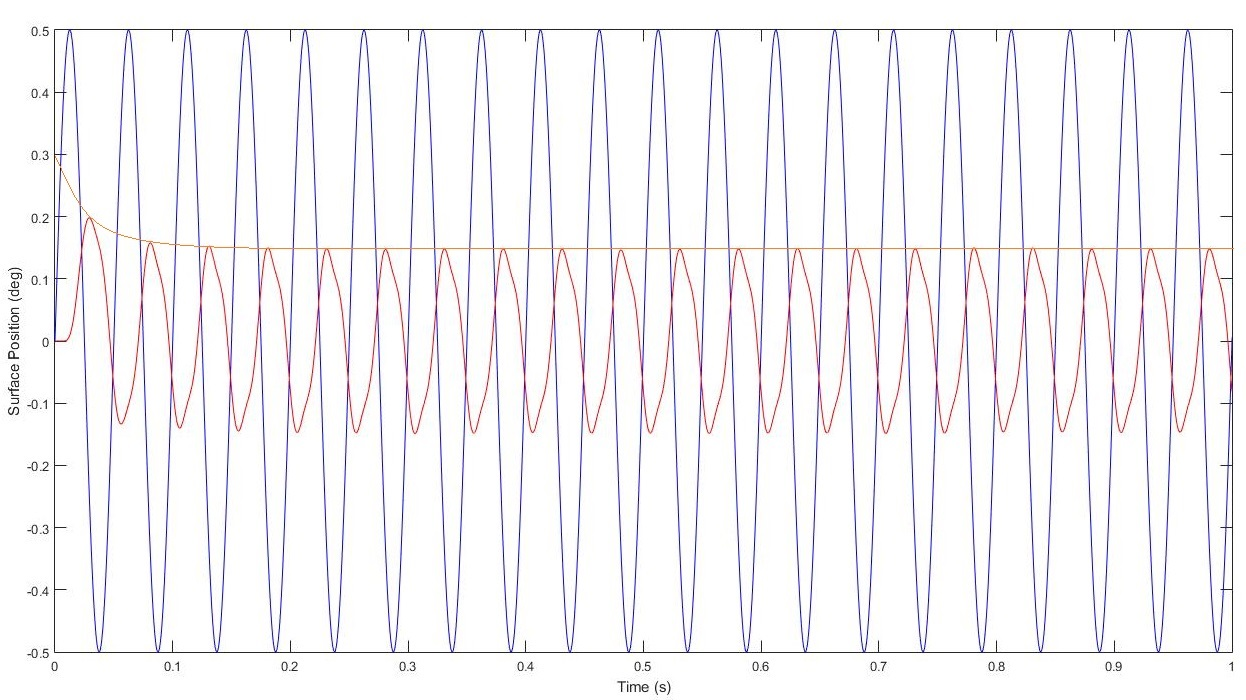
\includegraphics[width=0.9\textwidth]{Figuras/4.DynamicStifinessOptimizationAlgorithm/4-3-2-1-20HzTimeResponse.jpg}}
	\caption{20 Hz Sine Input System Response }
	\label{fig:4_3_2_1_20HzTimeResponse}
\end{figure}

Figure \ref{fig:4_3_2_1_20HzTimeResponse} also shows that for a pure sinusoidal input the output of the model is not a pure sinusoidal wave and therefore the system output is distorted and has harmonic components. This distortion is clearly observed in Figure \ref{fig:4_3_2_1_20HzTimeResponseZoom} which shows three cycles of the input after the dynamics have settled.

\begin{figure}[H]
	\centering
	\centerline{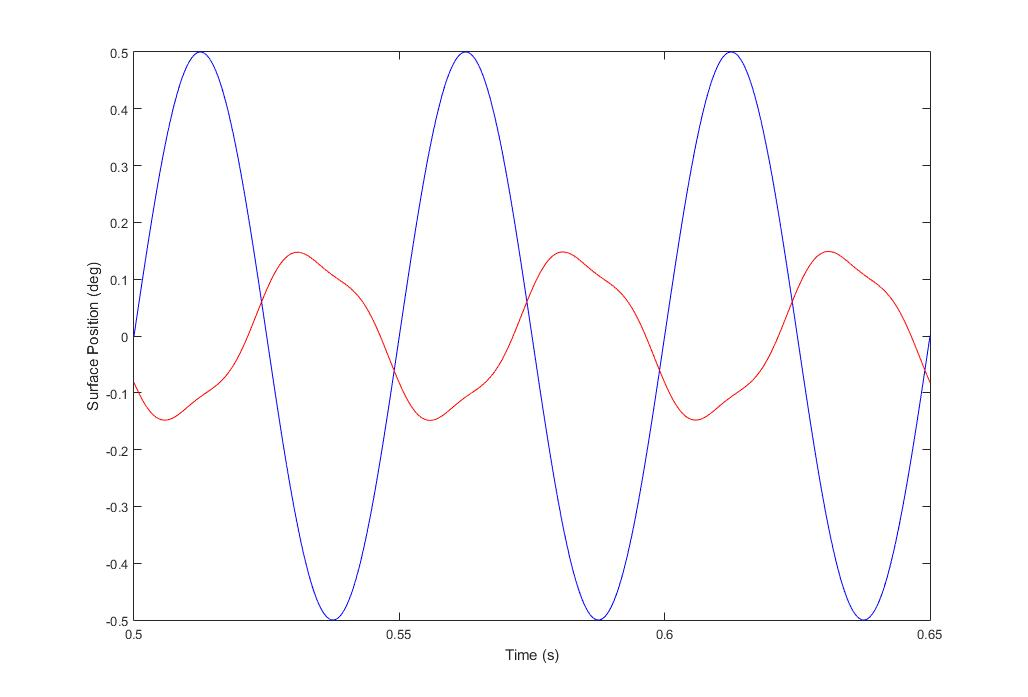
\includegraphics[width=0.9\textwidth]{Figuras/4.DynamicStifinessOptimizationAlgorithm/4-3-2-1-20HzTimeResponseZoom.jpg}}
	\caption{20 Hz Sine Input System Response }
	\label{fig:4_3_2_1_20HzTimeResponseZoom}
\end{figure}

Since the system output is distorted and therefore have harmonic components in its spectrum, it is required an analysis to assess if it is possible to consider only the component of the fundamental frequency in the calculation of the magnitude and phase of the output. The non-linearity at each frequency was evaluated by observing the respective THD as shown in Appendix \ref{NLFRAppendix}.

The FFT performed in the inputs and output signals did not consider the model dynamics settling time. Instead, it was performed for $K_{int}$ complete cycles from instant $T_{dyn}$ to the end of the simulation. A possible cause for the difference observed between the baseline and modified tests is that the baseline test considers all frequency cycles simulated, including those in the dynamics settling period whereas the modified test considers only the cycles after the dynamics have settled. When the first cycles are contained in the FFT data the result is affected by the different amplitude value observed in them. Both tests consider whole cycles for FFT data selection.

A comparison between the baseline and modified tests is presented in Figure \ref{fig:4_3_2_4_ModifiedBaselineScriptResults}. The figure shows that magnitude and phase responses for both tests match in most frequencies. Even though there is a difference between the curves at around 13 Hz, the overall response of the modified test is suitable for constraint evaluation purposes. It is important to remark that the baseline test is still used to evaluate initial and optimized controllers prior and after optimization.

\begin{figure}[H]
	\centering
	\centerline{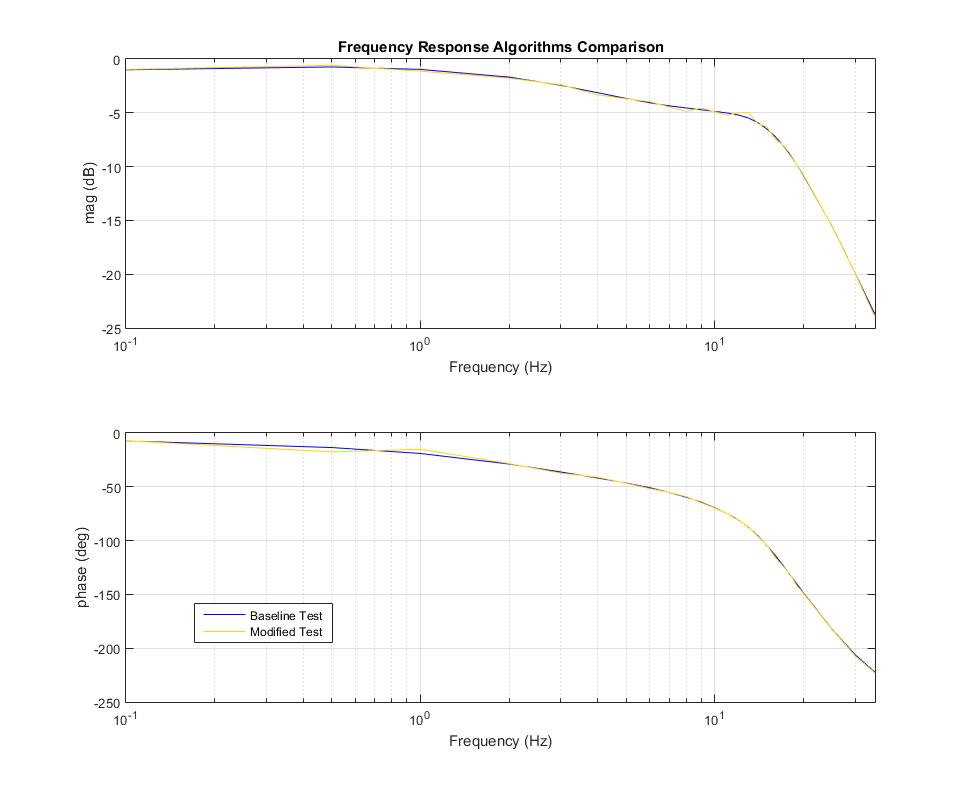
\includegraphics[width=0.9\textwidth]{Figuras/4.DynamicStifinessOptimizationAlgorithm/4-3-2-4-ModifiedBaselineScriptResults.jpg}}
	\caption{Baseline and Modified Frequency Response Test Results Comparison}
	\label{fig:4_3_2_4_ModifiedBaselineScriptResults}
\end{figure}

Table \ref{table:4_3_2_3_ModifiedBaselineScriptResults} shows that the closed-loop gain and phase allowances for both tests are the same and that bandwidth slightly increases. Also, execution time reduced by approximately 60\%, falling from 12.6 to 4.9 minutes.

\begin{table}[H]
	\captionof{table}{Baseline and Modified Frequency Response Test Results Comparison}
	\label{table:4_3_2_3_ModifiedBaselineScriptResults}
	\centering
	\resizebox{8cm}{!}{
		\begin{tabular}{|l|c|c|c|c|}
			\hline
			Constraint 							& Baseline 	& Modified 			\\ \hline
			Closed-Loop Gain Allowance (dB) 		& $13.0$	& $13.0$			\\ \hline
			Closed-Loop Phase Allowance ($°$)		& $Inf$  	& $Inf$	  			\\ \hline
			Closed-Loop Bandwidth (Hz) 			& $5.8$  	& $6.0$				\\ \hline
			Execution Time (min)				& $12.6$	& $4.9$				\\ \hline
	\end{tabular}}
\end{table}

Therefore, the modified test is a valid alternative to obtain the closed-loop frequency response of the actuation system since it yields a fairly similar response in much less time. This alternative test was used solely to evaluate optimization constraints. To evaluate the frequency performance of initial and optimized controllers the baseline test is still employed.

\section{Objective Function} \label{4-4-ObjectiveFunction}

The objective function $f(x)$ is responsible for conveying the fitness of a solution to a scalar value that will be minimized by the optimization algorithm. The output of the objective function is obtained by performing a dynamic stiffness test and calculating the cost function. These steps are described in the following sections.

\subsection{Dynamic Stiffness Test} \label{4-4-1-DynStiffTest}

The dynamic stiffness is obtained similarly to the frequency response, through simulation of the model for each evaluated frequency and further processing of the data generated by these simulations. Figure \ref{fig:4_4_1_DynamicStiffnessTestFlowchart} shows the flowchart of this test.

\begin{figure}[H]
	\centering
	\centerline{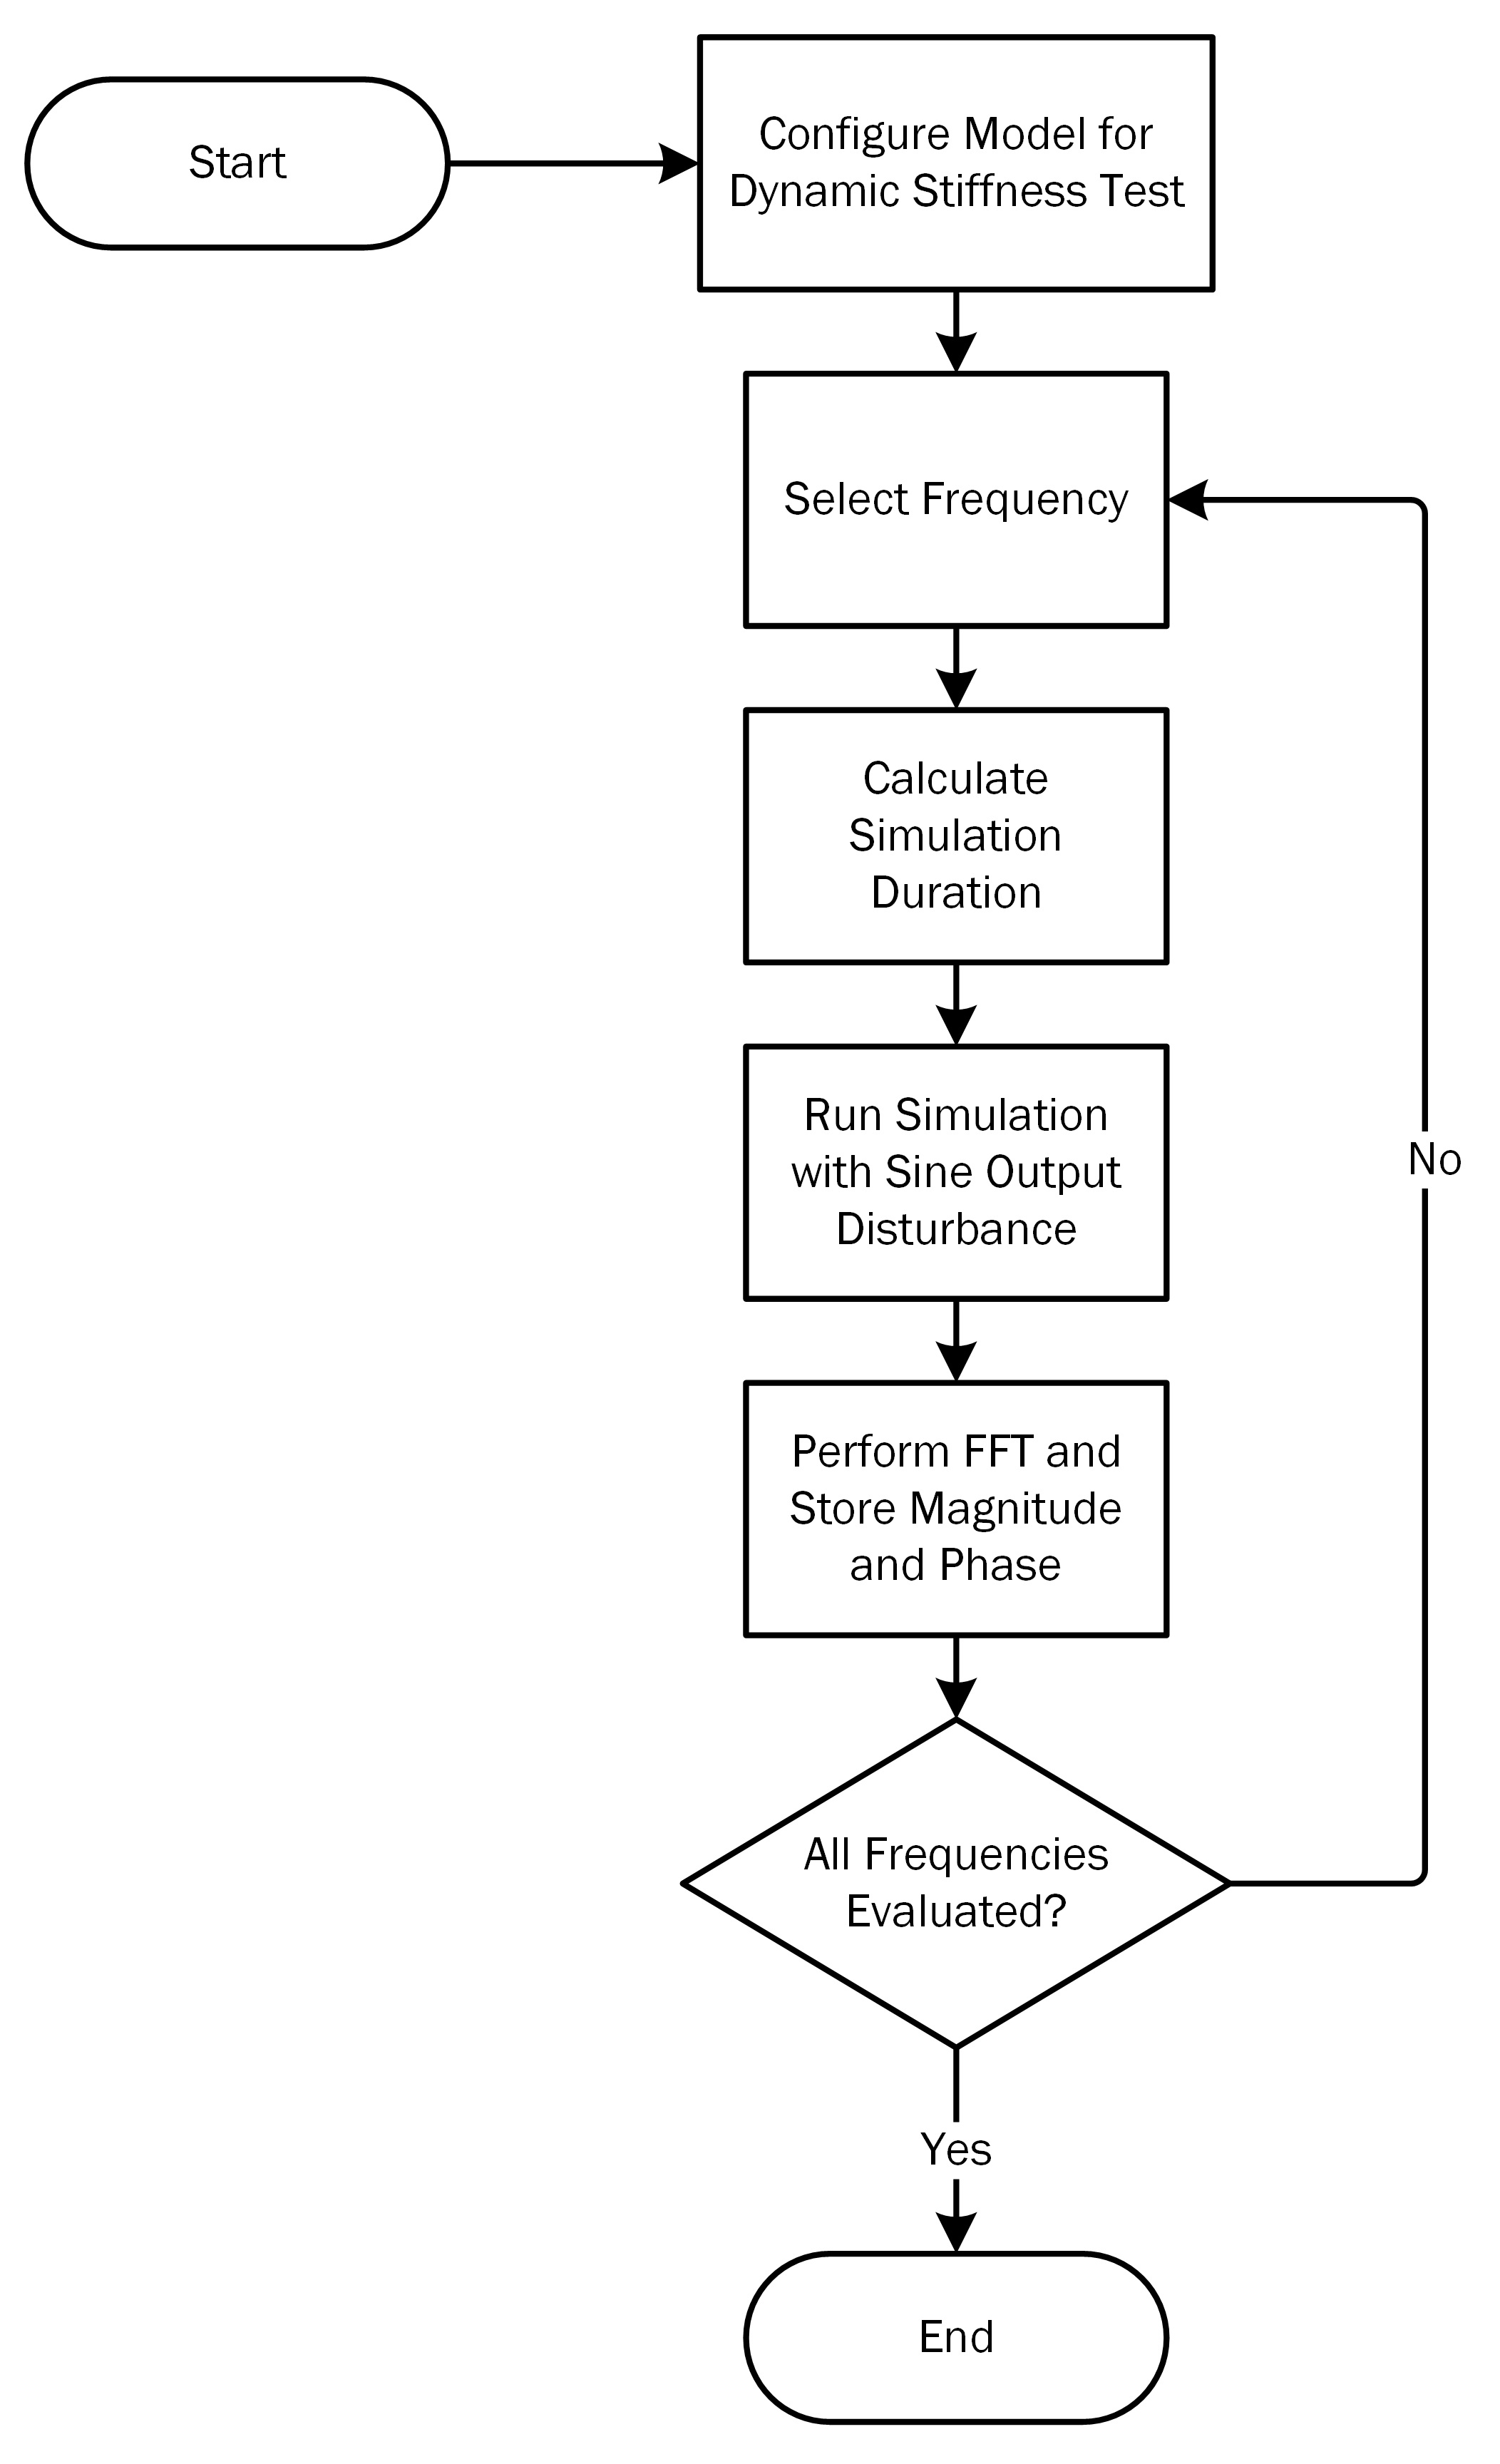
\includegraphics[width=0.6\textwidth]{Figuras/4.DynamicStifinessOptimizationAlgorithm/4-4-1-DynamicStiffnessTest.jpg}}
	\caption{Dynamic Stiffness Test Flowchart}
	\label{fig:4_4_1_DynamicStiffnessTestFlowchart}
\end{figure}

First, the model is configured to the following test condition:

\begin{enumerate}[a)]
	\item Single actuator connected to rudder surface;	
	\item Initial position = 0$°$;
	\item Position command = 0$°$;
	\item Sinusoidal aerodynamic load disturbance between 0.1 and 0.5 of actuator stall load;
	\item Maximum hydraulic supply pressure of 3000 psi;
	\item Maximum hydraulic return pressure of 150 psi;	
	\item At 100$°C$ (212$°F$) fluid temperature.	
\end{enumerate}

The test is performed with the highest fluid temperature of the operational envelope because, since the bulk modulus decreases when temperature rises, the fluid compressibility increases and that leads to lower dynamic stiffness. Since there is no surface command,  the flow in the cylinder chamber is not substantial and therefore the fluid density does not have a major influence in the response. Therefore, it is more conservative to evaluate actuator dynamic stiffness at 100$°C$. This behavior will be evident in chapter \ref{Optimization Results}.

Next, the aerodynamic load disturbance frequency to be evaluated is selected and the simulation duration period is calculated with the same method used in the baseline frequency response test. For frequencies up to 1 Hz, the duration spans for 3 complete sine cycles and, for frequencies between 1 Hz and 35 Hz, the number of cycles covered by the simulation is 3 times the evaluated frequency.

After that, the simulation is performed and the sinusoidal load disturbance and the ram position values are stored. This information is processed in the next step, when a FFT is performed for both signals. The transformed vectors are divided by each other and the real part of the resulting value at the excitation frequency yields the dynamic stiffness. The last steps are repeated until the dynamic stiffness is obtained for all frequencies of interest.

The execution time of the presented dynamic stiffness test is approximately 10 minutes which is a considerable computational cost. However, because this test is similar to the frequency response test, it is possible to implement the same modifications of the frequency response test in the dynamic stiffness test. 

Hence, the dynamic stiffness test was modified and the duration of each simulation is now calculated with equation \ref{eq:4_3_2_3_SimulationDuration}. This modification also excludes the effect of the model dynamics settling time in the actuator dynamic stiffness response. The same values of $K\textsubscript{int}$ for each frequencies were used. 

A comparison between both tests is shown in Figure \ref{fig:4_4_1_DynamicStiffnessComparison}. The yellow curve shows the dynamic stiffness obtained from the modified test which is fairly similar to the one from the original test, in blue. 

Therefore, the modified test can be used to evaluate the dynamic stiffness during optimization in order to reduce execution time which was reduced by approximately 43\%. Despite this, the original dynamic stiffness test is still employed to obtain this characteristic of the initial and final solutions of the optimization.

\begin{figure}[H]
	\centering
	\centerline{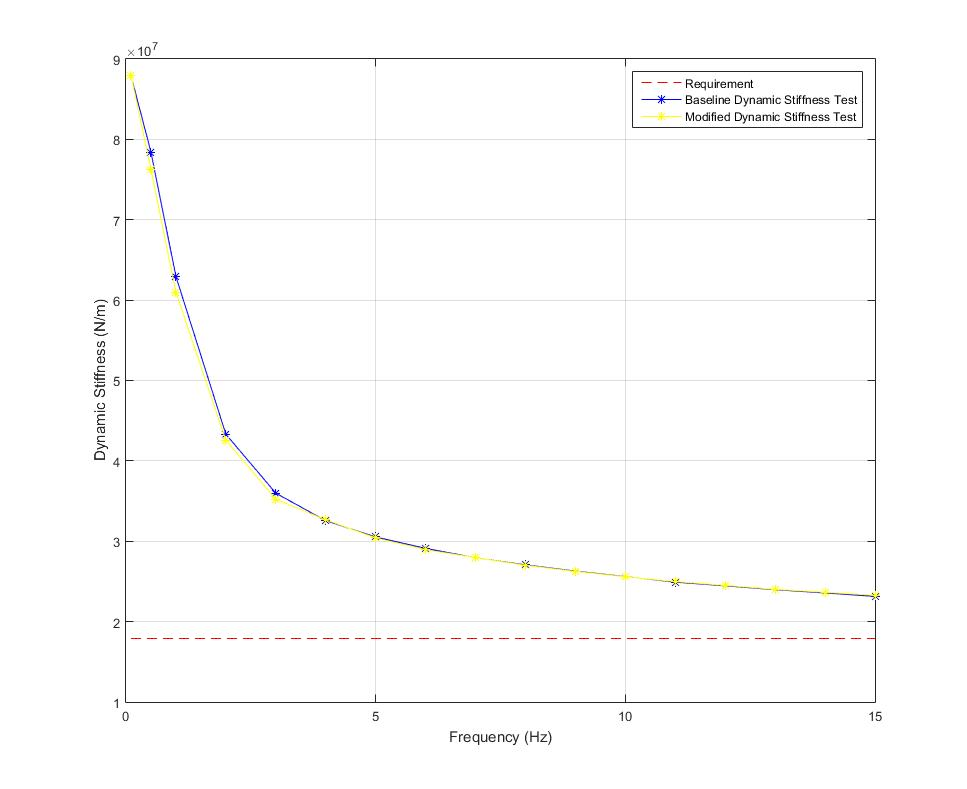
\includegraphics[width=0.9\textwidth]{Figuras/4.DynamicStifinessOptimizationAlgorithm/4-4-1-DynamicStiffnessComparison.jpg}}
	\caption{Baseline and Modified Dynamic Stiffness Test Comparison}
	\label{fig:4_4_1_DynamicStiffnessComparison}
\end{figure}

\subsection{Cost Function} \label{4-3-2-CostEquation}

After obtaining the dynamic stiffness response it is possible to calculate the cost function. Initially, a simple approach was considered as described by equations \ref{eq:4_4_2_CostEquation} and \ref{eq:4_4_2_PartialCostEquation}.

\begin{equation}
\label{eq:4_4_2_CostEquation}
f_1(x) = -( J_1(x) + J_2(x) + ... + J_i(x))
\end{equation} 

\begin{equation}
\label{eq:4_4_2_PartialCostEquation}
J_i(x) = K\textsubscript{act}(x,w_i) - K\textsubscript{req}
\end{equation} 

Where:

\begin{description}
	\item \hspace{20pt}$w_i$: i\textsuperscript{th} frequency evaluated;
	\item \hspace{20pt}$J_i(x)$: partial cost function related to the i\textsuperscript{th} frequency evaluated;
	\item \hspace{20pt}$K\textsubscript{act}$: actuation system dynamic stiffness for a given frequency;
	\item \hspace{20pt}$K\textsubscript{req}$: dynamic stiffness requirement.
\end{description}

Function $f_1(x)$ is a sum of several partial values related to each evaluated frequency in the system. These partial values are the difference between the dynamic stiffness value and the requirement at each frequency. Because the objective function is minimized during optimization, it must return a negative value in order to be maximized, hence the minus signal before the sum.

A second, more complex, cost function was considered in this work. Function $K$, proposed by \citeonline{Andersson} for multi-objective optimization in engineering design is represented as:

\begin{equation}
\label{eq:4_4_2_AnderssonEquation}
K = \left[\left( \frac{k_1}{k\textsubscript{10}} \right)^{\gamma_1} +
		  \left( \frac{k_2}{k\textsubscript{20}} \right)^{\gamma_2} + ... + 
		  \left( \frac{k_i}{k\textsubscript{i0}} \right)^{\gamma_i} \right] \times
		 [(1+c_1)^{\alpha_1} + (1+c_2)^{\alpha_2} + ... + (1+c_j)^{\alpha_j}]
\end{equation}

Where:

\begin{description}
	\item \hspace{20pt}$k_i$: sub function of G that expresses a characteristic of the system dependent on the optimization parameters;
	\item \hspace{20pt}$k\textsubscript{i0}$: sub function value for an acceptable solution;
	\item \hspace{20pt}$\gamma_i$: weight that represents the relative importance of each sub function;
	\item \hspace{20pt}$c_j$: constraint parameter equal to zero if j\textsuperscript{th} constraint is not violated or considerably greater than one otherwise;
	\item \hspace{20pt}$\alpha_j$: weight that represents the strength of each constraint.
\end{description}

This function provides flexibility to prioritize sub functions and better guide the optimization process. It also provides the possibility to incorporate penalization for constraint violation in the cost function value. Initially, it was implemented without the terms related to the problem constraints as shown in Equation \ref{eq:4_4_2_WeightedEquation}.

\begin{equation}
\label{eq:4_4_2_WeightedEquation}
f_2(x) = - \left[\left(\frac{J_1(x)}{J\textsubscript{10}} \right)^{\gamma_1} + 
		         \left(\frac{J_2(x)}{J\textsubscript{20}} \right)^{\gamma_2} + ... + 
		    	 \left(\frac{J_i(x)}{J\textsubscript{i0}} \right)^{\gamma_i}\right]
\end{equation}

In this case, $J_i(x)$ remains defined by Equation \ref{eq:4_4_2_PartialCostEquation}, $J\textsubscript{i0}$ is the partial value for a dynamic stiffness marginally above the requirement and $\gamma_i$ is a weight dependent on the frequency. A $\gamma_i$ of 5 was considered for the infinite frequency and 1 otherwise.

However, this implementation was not robust against constraint violation. The results obtained using this approach did not satisfy the performance requirements implemented using the constraint function described in section \ref{4-3-ConstraintFunction}.

To overcome this issue, function $f_2(x)$ was modified to include penalties for not meeting required performance. The updated function is shown in Equation \ref{eq:4_4_3_ContrainedWeightedEquation}.

\begin{equation}
\label{eq:4_4_3_ContrainedWeightedEquation}
f_2(x) = - \left[\left( \frac{J_1(x)}{J\textsubscript{10}} \right)^{\gamma_1} + 
		    	 \left( \frac{J_2(x)}{J\textsubscript{20}} \right)^{\gamma_2} + ... + 
		    	 \left( \frac{J_i(x)}{J\textsubscript{i0}} \right)^{\gamma_i} \right]+
		 	 	 [(1+r_1)^{\alpha_1} + (1+r_2)^{\alpha_2} + ... + (1+r_j)^{\alpha_j}]
\end{equation}

Where $r_j$ is the result of the evaluation of the j\textsuperscript{th} constraint. If the constraint complies with the requirement $r_j$ equals zero otherwise $r_j$ is the difference between the constraint and the requirement. Also, $\alpha_j$ is the weight that represents the strength of this constraint. In this case, $\alpha_j$ was arbitrated as 5 for all constraints. Finally, the constraint polynomial is summed to the objective polynomial instead of multiplied. This modification was necessary because multiplying would benefit instead of penalizing the inadequate solution.

Finally, both cost functions $f_1(x)$ and $f_2(x)$ have another component intended to avoid evaluation of solutions that do not meet the dynamic stiffness requirement: if the requirement is not met at any evaluated frequency, a component substantially greater than the cost function is added turning $f_1(x)$ and $f_2(x)$ into large positive values.

The next chapter presents the optimization results obtained with each function.